\documentclass[11pt, a4paper, DIV=12]{scrartcl}

% useful packages 
\usepackage{mathtools}
\usepackage{physics}
\usepackage{graphicx}					  
\graphicspath{{figs/}}



\usepackage{amssymb}
\usepackage{amsmath}
\usepackage{hyperref}
\usepackage[separate-uncertainty=true]{siunitx}
\usepackage{xcolor}
\usepackage{braket} % easy braket notation
\usepackage{enumitem}
\usepackage{booktabs}
\usepackage{here}
\usepackage{cprotect}

\usepackage[backend=biber, sorting=none]{biblatex}
\bibliography{refs.bib}

% \numberwithin{equation}{section}

\title{Error analysis of a Markov Chain}
\date{\today}
\author{Harilal Bhattarai \& Marcel Schindler}
\begin{document}
	\maketitle
	
\section{Introduction}
In this week’s exercise we apply proper analysis techniques to estimate the statistical error of a quantity estimated from a Markov Chain (MC).
\section{Theory}
The Markov Chain has reached the equilibrium distribution we use the usual ensemble mean
\begin{equation}
\bar{m}_{N}= \frac{1}{N}\sum_{k=1}^{N} m(\phi_{k})
\end{equation}
as the Monte-Carlo estimator of the magnetization $ <m> $.\\

\textbf{Autocorrelation}\\
\textbf{Blocking}: It is also called binning.\\
\textbf{The bootstrap}

\section{Analysis}
To compare the two MC trajectories, we set $\beta \text{J}= 0.1 $; $\beta \text{h}= 0.5 $; n=5; for two different number of integration steps $ N_{md}=4$ and  $\text{N}_{md}= 100 $. we generate long MC for each run $ \text{N}=12800 $.

\begin{figure}[H]
	\centering
	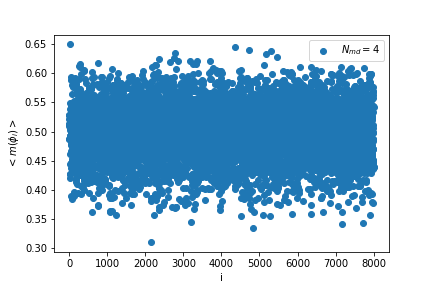
\includegraphics[width=0.6\linewidth]{comparison_magnitization_4.png}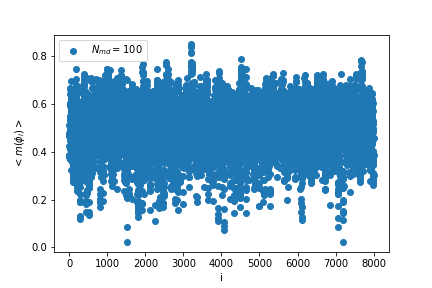
\includegraphics[width=0.6\linewidth]{comparison_magnitization_100.png}
	\caption{Trajectories of the MC history of magnetization with different number of integration steps. Here, two graphs are at $ N_{md}=4$ and $ N_{md}=100$.}
	\label{fig:comperison}
\end{figure}
\textbf{Autocorrelation}

\begin{figure}[H]
	\centering
	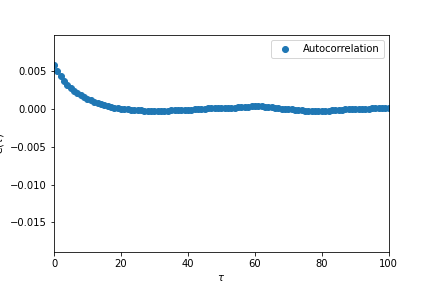
\includegraphics[width=0.6\linewidth]{autokorrelation.png}
	\caption{Plot of the function of straightforward estimator $ C(\tau) $ to generated data sets.}
	\label{fig:autocorrelation}
\end{figure}

\textbf{Blocking}: It is also called binning.
\begin{figure}[H]
	\centering
	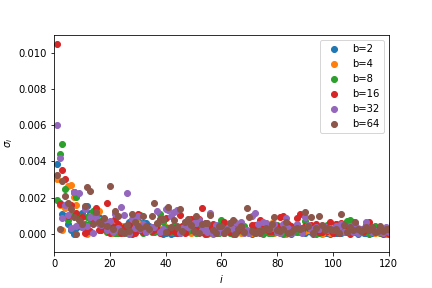
\includegraphics[width=0.6\linewidth]{blocking_standard_deviation.png}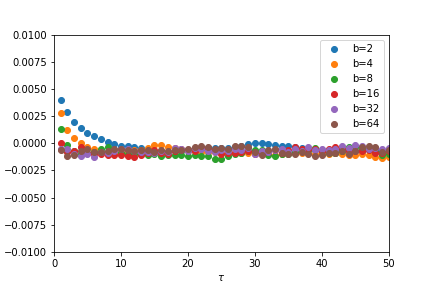
\includegraphics[width=0.6\linewidth]{blocking_autokorrelation.png}
	\caption{ The autocorrelation for blocked data for b= 2, 4, 8, 16, 32, and 64.}
	\label{fig:blockingAutocorrelation}
\end{figure}

\textbf{The bootstrap}	
\begin{figure}[H]
	\centering
	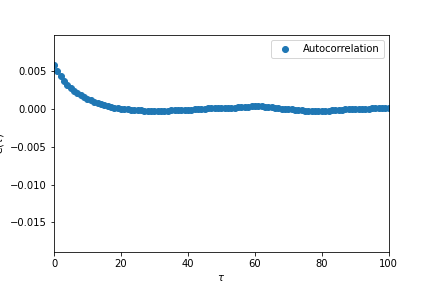
\includegraphics[width=0.6\linewidth]{autokorrelation.png}
	\caption{ The stability of the error as a function of $ N_{bs} $ .}
	\label{fig:boottrap}
\end{figure}	
	\begin{thebibliography}{12}
		\bibitem{exercise-sheet} 
		Thomas Luu, Andreas Nogga, Marcus Petschlies and  Andreas Wirzba, Exercise-sheet, 2020. 
		
		
	\end{thebibliography}	
\end{document}